\chapter{Constraint Satisfaction}
In this chapter we discuss algorithms for solving \emph{\color{blue}constraint satisfaction problems}.
This chapter is structured as follows:
\begin{enumerate}
\item The first section defines the notion of a constraint satisfaction problem.  In order to illustrate this
      concept, two examples of constraint satisfaction problems are presented.  After that, we discuss
      applications of constraint satisfaction problems.
\item The simplest algorithm to solve a constraint satisfaction problem is via \emph{\color{blue}Backtracking Search}.
      This is presented in Section 2.
\item Backtracking Search can be refined to \emph{\color{blue}Non-Chronological Backtracking}, which is presented in
      Section 3.
\item Finally, the last section shows how constraint satisfaction problems can be solved via
      \emph{\color{blue}local search}.
\end{enumerate}

\section{Formal Definition of Constraint Satisfaction Problems}
Formally, we define a 
\href{https://en.wikipedia.org/wiki/Constraint_satisfaction_problem}{constraint satisfaction problem} as a triple
\\[0.2cm]
\hspace*{1.3cm}
$\mathcal{P} := \langle \mathtt{Vars}, \mathtt{Values}, \mathtt{Constraints} \rangle$
\\[0.2cm]
where
\begin{enumerate}
\item $\mathtt{Vars}$ is a set of strings which serve as \emph{variables},
\item $\mathtt{Values}$ is a set of \emph{values} for the variables in $\mathtt{Vars}$.
\item $\mathtt{Constraints}$ is a set of formulae from \emph{\color{blue}first order logic}.  Each of these formulae is
      called a \emph{\color{blue}constraint} of $\mathcal{P}$.

      In order to be able to interpret these formulae, we need a $\emph{first order structure}$ $\mathcal{S} = \langle \mathcal{U}, \mathcal{J} \rangle$.  
      Here, $\mathcal{U}$ is the $\emph{\color{blue}universe}$ of $\mathcal{S}$ and we will assume that this
      universe is identical to the set $\mathtt{Values}$. The second component $\mathcal{J}$ is the
      \emph{\color{blue}interpretation} of the function symbols and predicate symbols that are used in the 
      constraints.  In what follows we assume that this interpretation is understood from the context of the
      constraint satisfaction problem $\mathcal{P}$.
\end{enumerate}
In the following, the abbreviation \textsc{Csp} is short for \emph{\color{blue}constraint satisfaction problem}.
Given a \textsc{Csp}
\\[0.2cm]
\hspace*{1.3cm}
 $\mathcal{P} = \langle \mathtt{Vars}, \mathtt{Values}, \mathtt{Constraints} \rangle$, 
\\[0.2cm]
a \emph{\color{blue}variable assignment} for $\mathcal{P}$ is a function
\\[0.2cm]
\hspace*{1.3cm}
$A: \mathtt{Vars} \rightarrow \mathtt{Values}$.
\\[0.2cm]
A variable assignment $A$ is a \emph{\color{blue}solution} of the \textsc{Csp} $\mathcal{P}$ 
if, given the assignment $A$, all constraints of $\mathcal{P}$ are satisfied.
We proceed to illustrate the definitions given so far with two examples.


\begin{figure}[!ht]
  \centering
  \framebox{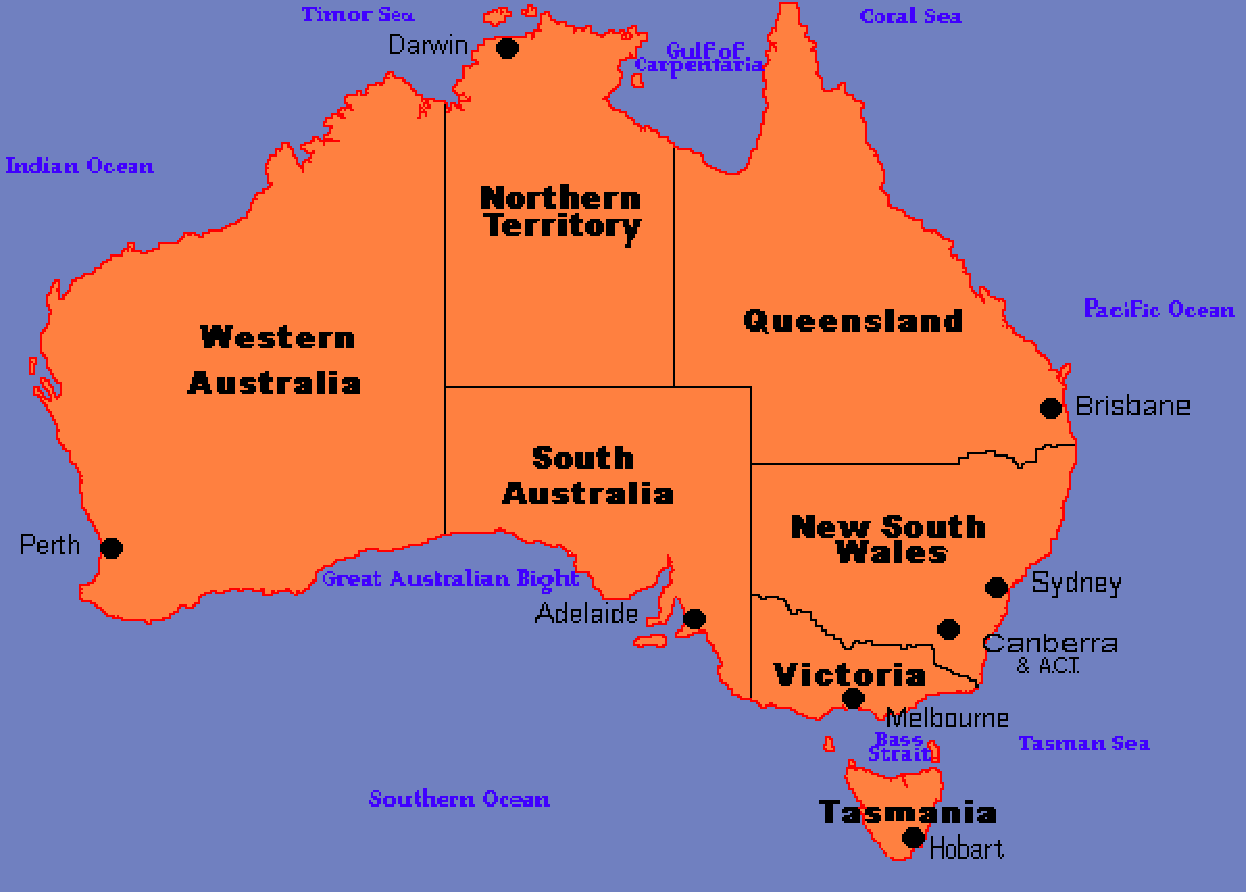
\epsfig{file=Figures/australia.pdf,scale=0.8}} 
  \caption{A map of Australia.}
  \label{fig:australia.pdf}
\end{figure}

\subsection{Example: Map Coloring}
In \href{https://en.wikipedia.org/wiki/Four_color_theorem}{map colouring} a map showing different state
borders is given and the task is to colour the different states such that no two states that have a common
border share the same colour.  \myFig{australia.pdf} shows a map of Australia.  There are seven different
states in Australia:
\begin{enumerate}
\item Western Australia, abbreviated as $\mathrm{WA}$,
\item Northern Territory, abbreviated as $\mathrm{NT}$,
\item South Australia, abbreviated as $\mathrm{SA}$,
\item Queensland, abbreviated as $\mathrm{Q}$,
\item New South Wales, abbreviated as $\mathrm{NSW}$,
\item Victoria, abbreviated as $\mathrm{V}$, and
\item Tasmania, abbreviated as $\mathrm{T}$.
\end{enumerate}
Figure \ref{fig:australia.pdf} would certainly look better if different states had been coloured with different
colours.  For the purpose of 
this example let us assume that we have only three colours available.  The question then is whether it is 
possible to colour the different states in a way that no two neighbouring states share the same colour.  This
problem can be formalized as a constraint satisfaction problem.  To this end we define:
\begin{enumerate}
\item $\mathtt{Vars} := \{ \mathrm{WA}, \mathrm{NT}, \mathrm{SA}, \mathrm{Q}, \mathrm{NSW}, \mathrm{V}, \mathrm{T} \}$,
\item $\mathtt{Values} := \{ \mathtt{red}, \mathtt{green}, \mathtt{blue} \}$,
\item $\mathtt{Constraints} := 
         \bigl\{ \mathrm{WT} \not= \mathrm{NT}, \mathrm{WT} \not= \mathrm{SA},
                 \mathrm{NT} \not= \mathrm{SA}, \mathrm{NT} \not= \mathrm{Q},
                 \mathrm{SA} \not= \mathrm{Q}, \mathrm{SA} \not= \mathrm{NSW}, \mathrm{SA} \not= \mathrm{V}, 
                 \mathrm{V} \not = \mathrm{T}
         \bigr\}
        $
\end{enumerate}
Then $\mathcal{P} := \langle \mathtt{Vars}, \mathtt{Values}, \mathtt{Constraints} \rangle$ is a constraint satisfaction problem.  
If we define the assignment $A$ such that
\begin{enumerate}
\item $A(\mathrm{WA}) = \mathtt{blue}$,
\item $A(\mathrm{NT}) = \mathtt{red}$,
\item $A(\mathrm{SA}) = \mathtt{green}$,
\item $A(\mathrm{Q}) = \mathtt{blue}$,
\item $A(\mathrm{NSW}) = \mathtt{red}$,
\item $A(\mathrm{V}) = \mathtt{blue}$,
\item $A(\mathrm{T}) = \mathtt{red}$,
\end{enumerate}
then you can check that the assignment $A$ is indeed a solution to the constraint satisfaction problem $\mathcal{P}$.

\subsection{Example: The Eight Queens Puzzle}
The \href{https://en.wikipedia.org/wiki/Eight_queens_puzzle}{eight queens problem} asks to put 8 queens onto a
chessboard such that no queen can attack another queen.  In \href{https://en.wikipedia.org/wiki/Chess}{chess},
a queen can attack all pieces that are either in the same row, the same column, or the same diagonal.  If we
want to put 8 queens on a chessboard such that no two queens can attack each other, we have to put exactly one
queen in every row:  If we would put more than one queen in a row, the queens in that row can attack each other.
If we would leave a row empty, then, given that the other rows contain at most one queen, there would be less
than 8 queens on the board.  Therefore, in order to model the eight queens problem as a constraint satisfaction
problem, we will use the following set of variables:
\\[0.2cm]
\hspace*{1.3cm}
$\mathtt{Vars} := \{ \mathtt{V}_1, \mathtt{V}_2, \mathtt{V}_3, \mathtt{V}_4, \mathtt{V}_5, \mathtt{V}_6, \mathtt{V}_7,\mathtt{V}_8 \}$,
\\[0.2cm]
where for $i \in \{1,\cdots,8\}$ the variable $\mathtt{V}i$ specifies the column of the queen that is placed in
row $i$.   As the columns run from one to eight, we define the set $\mathtt{Values}$ as
\\[0.2cm]
\hspace*{1.3cm}
$\mathtt{Values} := \{1,2,3,4,5,6,7,8\}$.
\\[0.2cm]
Next, let us define the constraints.  There are three different types of constraints.
\begin{enumerate}
\item We have constraints that express that no two queens positioned in different rows share the same column.
      To capture these constraints, we define
      \\[0.2cm]
      \hspace*{1.3cm}
      $\mathtt{SameRow} := \bigl\{ \mathtt{V}_i \not= \mathtt{V}_j \bigm| i \in \{1,\cdots,8\} \wedge j \in \{1,\cdots,8\} \wedge j < i \bigr\}$.
      \\[0.2cm]
      Here the condition $i < j$ ensures that, for example, we have the constraint $\mathtt{V}_2 \not= \mathtt{V}_1$
      but not the constraint  $\mathtt{V}_1 \not= \mathtt{V}_2$, as the latter would be redundant if the former is
      already given.
\item We have constraints that express that no two queens positioned in different rows share the same rising
      diagonal.  To capture these constraints, we define
      \\[0.2cm]
      \hspace*{1.3cm}
      $\mathtt{SameRising} := \bigl\{ i + \mathtt{V}_i \not= j + \mathtt{V}_j \bigm| i \in \{1,\cdots,8\} \wedge j \in \{1,\cdots,8\} \wedge j < i \bigr\}$.
\item We have constraints that express that no two queens positioned in different rows share the same falling
      diagonal.  To capture these constraints, we define
      \\[0.2cm]
      \hspace*{1.3cm}
      $\mathtt{SameFalling} := \bigl\{ i - \mathtt{V}_i \not= j - \mathtt{V}_j \bigm| i \in \{1,\cdots,8\} \wedge j \in \{1,\cdots,8\} \wedge j < i \bigr\}$.
\end{enumerate}
Then, the set of constraints is defined as 
\\[0.2cm]
\hspace*{1.3cm}
$\mathtt{Constraints} := \mathtt{SameRow} \cup \mathtt{SameRising} \cup \mathtt{SameFalling}$
\\[0.2cm]
and the eight queens problem can be stated as the constraint satisfaction problem
\\[0.2cm]
\hspace*{1.3cm}
$\mathcal{P} := \langle \mathtt{Vars}, \mathtt{Values}, \mathtt{Constraints} \rangle$.
\\[0.2cm]
If we define the assignment $A$ such that
\\[0.2cm]
\hspace*{1.3cm}
$A(1) := 4,\; A(2) := 8,\; A(3) := 1,\; A(4) := 2,\; A(5) := 6,\; A(6) := 2,\; A(7) := 7,\; A(8) := 5$,
\\[0.2cm]
then it is easy to see that this assignment is a solution of the eight queens problem.  This solution is shown
in \myFig{eight-queens.txt}.


\begin{figure}[!ht]
  \centering
\hspace*{0.0cm}
\vbox{\offinterlineskip
   \hrule height1pt
   \hbox{\vrule width1pt\bigchess
         \vbox{\hbox{0Z0L0Z0Z}
               \hbox{Z0Z0Z0ZQ}
               \hbox{QZ0Z0Z0Z}
               \hbox{Z0L0Z0Z0}
               \hbox{0Z0Z0L0Z}
               \hbox{ZQZ0Z0Z0}
               \hbox{0Z0Z0ZQZ}
               \hbox{Z0Z0L0Z0}}%
         \vrule width1pt}
   \hrule height1pt}

  \caption{Eine L\"{o}sung des 8-Damen-Problems.}
  \label{fig:eight-queens.txt}
\end{figure}


\myFig{queens-csp.stlx} shows a \textsc{SetlX} program that can be used to create the eight queens puzzle as a
\textsc{Csp}.  The code shown in this figure is more general than the eight queens puzzle:  Given a natural
number $n$, the function call $\mathtt{queensCSP}(n)$ creates a constraint satisfaction problem $\mathcal{P}$ that generalizes
the eight queens problem to the problem of putting $n$ queens on a board of size $n$ times $n$.

\begin{figure}[!ht]
\centering
\begin{Verbatim}[ frame         = lines, 
                  framesep      = 0.3cm, 
                  firstnumber   = 1,
                  labelposition = bottomline,
                  numbers       = left,
                  numbersep     = -0.2cm,
                  xleftmargin   = 0.8cm,
                  xrightmargin  = 0.8cm,
                ]
    queensCSP := procedure(n) {
        Variables   := { "V$i$" : i in {1..n} };
        Values      := { 1 .. n };
        Constraints := {};
        for (i in [2..n], j in [1..i-1]) {
            Constraints += { "V$i$ != V$j$" };
            Constraints += { "$i$ + V$i$ != $j$ + V$j$" };
            Constraints += { "$i$ - V$i$ != $j$ - V$j$" };
        }
        return [Variables, Values, Constraints];
    };
\end{Verbatim}
\vspace*{-0.3cm}
\caption{\textsc{SetlX} code to create the CSP representing the eight-queens puzzle.}
\label{fig:queens-csp.stlx}
\end{figure}

The beauty of \href{https://en.wikipedia.org/wiki/Constraint_programming}{constraint programming} is the fact
that we will be able to develop a so called \emph{\color{blue}constraint solver} that takes as input a \textsc{Csp}
like the one produced by the program shown in Figure \ref{fig:queens-csp.stlx} and that is then capable of
computing a solution. 

\subsection{Applications}
Besides the toy problems discussed so far, there are a number of industrial applications of constraint
satisfaction problems.  The most important application seem to be variants of
\href{https://en.wikipedia.org/wiki/Scheduling_(production_processes)}{scheduling problems}. 
A simple example of a scheduling problem is the problem of generating a time table for a school.  A school has
various teachers, each of which can teach some subjects but not others.  Furthermore, there are a number of
classes that must be taught in different subjects.  The problem is then to assign teachers to classes and to
create a time table.
\pagebreak

\section{Backtracking Search}
\begin{figure}[!ht]
\centering
\begin{Verbatim}[ frame         = lines, 
                  framesep      = 0.3cm, 
                  firstnumber   = 1,
                  labelposition = bottomline,
                  numbers       = left,
                  numbersep     = -0.2cm,
                  xleftmargin   = 0.8cm,
                  xrightmargin  = 0.8cm,
                ]
    solve := procedure(csp) {
        [Vars, Vals, Constrs] := csp;
        csp := [Vars, Vals, { [f, collectVars(f)] : f in Constrs }];
        check {
            return bt_search({}, csp);
        }
    };
    bt_search := procedure(Assignment, csp) {
        [Variables, Values, Constraints] := csp;
        if (#Assignment == #Variables) {
            return Assignment;
        }
        var := select_unassigned_variable(Assignment, Variables);
        for (value in Values) {
            check {
                if (is_consistent(var, value, Assignment, Constraints)) {
                    return bt_search(Assignment + { [var, value] }, csp);
                }
            }
        }
        backtrack;
    };
\end{Verbatim}
\vspace*{-0.3cm}
\caption{A backtracking \textsc{Csp} solver.}
\label{fig:csp-backtrack-solver.stlx-1}
\end{figure}

\begin{figure}[!ht]
\centering
\begin{Verbatim}[ frame         = lines, 
                  framesep      = 0.3cm, 
                  firstnumber   = 1,
                  labelposition = bottomline,
                  numbers       = left,
                  numbersep     = -0.2cm,
                  xleftmargin   = 0.8cm,
                  xrightmargin  = 0.8cm,
                ]
    select_unassigned_variable := procedure(Assignment, Variables) {
        return rnd({ v : v in Variables | Assignment[v] == om });
    };
    eval_constraint := procedure(Assignment, Vars, Formula) {
        for (v in Vars) {
            execute("$v$ := $Assignment[v]$;");
        }
        return eval(Formula);
    };
    is_consistent := procedure(var, value, Assignment, Constraints) {
        for ([Formula, Vars] in Constraints | var in Vars) {
            NewAssignment := Assignment + { [var, value] };
            if (Vars <= domain(NewAssignment)) {
                if (!eval_constraint(NewAssignment, Vars, Formula)) {
                    return false;
                }
            }
        }
        return true;
    };
\end{Verbatim}
\vspace*{-0.3cm}
\caption{Auxiliary procedures for the \textsc{Csp} solver shown in Figure \ref{fig:csp-backtrack-solver.stlx-1}}
\label{fig:csp-backtrack-solver.stlx-2}
\end{figure}


\section{Non-Chronological Backtracking}
\section{Local Search}
There is another approach to solve constraint satisfaction problems.  This approach is known as
\emph{\color{blue}local search}.  The basic idea is simple: Given as constraint satisfaction problem 
$\mathcal{C}$ of the form 
\\[0.2cm]
\hspace*{1.3cm}
$\mathcal{C} := \langle V, C, D \rangle$,
\\[0.2cm] 
local search works as follows:
\begin{enumerate}
\item Initialize the values of the variables in $V$ randomly.  
\item If all constraints are satisfied, return the solution.
\item For every variable $x \in V$, count the number of \underline{unsatisfied} constraints that involve the
      variable $x$. 
\item Set $\mathtt{maxNum}$ to be the biggest number of unsatisfied constraints for a single variable.
\item Compute the set $\mathtt{maxVars}$ of those variables that have $\mathtt{maxNum}$ unsatisfied constraints.
\item Randomly choose a variable $x$ from the set $\mathtt{maxVars}$.
\item Find a value $d \in D$ such that by assigning $d$ to the variable $x$, the number of unsatisfied constraints is
      minimized.  

      If there is more than one value $d$ with this property, choose the value $d$ randomly from those values
      that minimize the number of unsatisfied constraints.
\item Goto step 2 and repeat until a solution is found.
\end{enumerate}

\begin{figure}[!ht]
\centering
\begin{Verbatim}[ frame         = lines, 
                  framesep      = 0.3cm, 
                  firstnumber   = 1,
                  labelposition = bottomline,
                  numbers       = left,
                  numbersep     = -0.2cm,
                  xleftmargin   = 0.8cm,
                  xrightmargin  = 0.8cm,
                ]
    solve := procedure(n) {
        Queens := [];
        for (row in [1 .. n]) {
            Queens[row] := rnd({1 .. n});
        }
        iteration := 0;
        while (true) {
            Conflicts   := { [numConflicts(Queens, row), row] : row in [1 ..n] };
            [maxNum, _] := last(Conflicts);
            if (maxNum == 0) {
                return Queens;
            }
            if (iteration % 10 != 0) { // avoid infinite loops
                row := rnd({ row : [num, row] in Conflicts | num == maxNum });
            } else {
                row := rnd({ 1 .. n });
            }
            Conflicts := {};
            for (col in [1 .. n]) {
                Board      := Queens;
                Board[row] := col;
                Conflicts  += { [numConflicts(Board, row), col] };
            }
            [minNum, _] := first(Conflicts);
            Queens[row] := rnd({ col : [num, col] in Conflicts | num == minNum });
            iteration   += 1;
        }
    };
\end{Verbatim}
\vspace*{-0.3cm}
\caption{Solving the $n$ queens problem using local search.}
\label{fig:constraints.stlx}
\end{figure}

\noindent
\myFig{constraints.stlx} shows an implementation of these ideas in \textsc{SetlX}.  Instead of solving an
arbitrary constraint satisfaction problem, the program solves the $n$ queens problem.  We proceed to discuss
this program line by line.
\begin{enumerate}
\item The procedure $\mathtt{solve}$ takes one parameter $\mathtt{n}$, which is the size of the chess board.  If
      the computation is successful, $\mathtt{solve(n)}$ returns a list of length $\mathtt{n}$.  Lets call this
      list $\mathtt{Queens}$. For every row $\mathtt{r} \in \{1, \cdots, \mathtt{n}\}$, the value $\mathtt{Queens[r]}$ specifies that the queen 
      that resides in row $\mathtt{r}$ is positioned in column $\mathtt{Queens[r]}$.
\item The \texttt{for} loop initializes the positions of the queens to random values from the set
      $\{1, \cdots, \mathtt{n}\}$.  Effectively, for every row on the chess board, this puts a queen in a
      random column.
\item The variable $\mathtt{iteration}$ counts the number of times that we need to reassign a queen in a given row.
\item All the remaining statements are surrounded by a \texttt{while} loop that is only terminated once a
      solution has been found.
\item The variable $\mathtt{Conflicts}$ is a set of pairs of the form $[c, r]$, where $c$ is the number of
      times the queen in row $r$ is attacked by other queens.  Hence, $c$ is the same as the number of
      unsatisfied conflicts for the variable specifying the column of the queen in row $r$.
\item $\mathtt{maxNum}$ is the maximum of the number of conflicts for any row.
\item If this number is $0$, then all constraints are satisfied and the list $\mathtt{Queens}$ is a solution to the
      $\mathtt{n}$ queens problem.
\item Otherwise, we compute those rows that exhibit the maximal number of conflicts.  From these rows
      we select one $\mathtt{row}$ arbitrarily.
\item The reason for enclosing the assignment to $\mathtt{row}$ in an \texttt{if} statement is explained later. 
      On a first reading of  this program,  this \texttt{if} statement should be ignored.
\item Now that we have identified the $\mathtt{row}$ where the number of conflicts is biggest, we need to
      reassign $\mathtt{Queens[row]}$.  Of course, when reassigning this variable, we would like to have fewer
      conflicts after the reassignment.  Hence, we test all columns to find the best column that can be
      assigned for the queen in the given $\mathtt{row}$.  This is done in a \texttt{for} loop that runs over
      all possible columns.  The set $\mathtt{Conflicts}$ that is maintained in this loop is a set of pairs
      of the form $[k, c]$ where $k$ is the number of times the queen in $\mathtt{row}$ would be attacked if it
      would be placed in column $c$.
\item We compute the minimum number of conflicts that is possible for the queen in $\mathtt{row}$ and assign it
      to $\mathtt{minNum}$.
\item From those columns that minimize the number of violated constraints, we choose a column randomly
      and assign it for the specified $\mathtt{row}$.
\end{enumerate}
There is a technical issue, that must be addressed:  It is possible there is just one row that exhibits the
maximum number of conflicts.  It is further possible that, given the placements of the other queens, there is
just one optimal column for this row.  In this case, the procedure $\mathtt{solve}$ would loop forever.  To
avoid this case, every 10 iterations we pick a random row to change.

\begin{figure}[!ht]
\centering
\begin{Verbatim}[ frame         = lines, 
                  framesep      = 0.3cm, 
                  firstnumber   = 1,
                  labelposition = bottomline,
                  numbers       = left,
                  numbersep     = -0.2cm,
                  xleftmargin   = 0.8cm,
                  xrightmargin  = 0.8cm,
                ]
    numConflicts := procedure(Queens, row) {
        n      := #Queens;
        result := 0;
        for (r in {1 .. n} | r != row) {
            if ( Queens[r] == Queens[row]           ||
                 r - Queens[r] == row - Queens[row] ||
                 r + Queens[r] == row + Queens[row]
               )
            { result += 1; }
        }
        return result;
    };
\end{Verbatim}
\vspace*{-0.3cm}
\caption{The procedure $\mathtt{numConficts}$.}
\label{fig:numConficts.stlx}
\end{figure}

The procedure $\mathtt{numConficts}$ shown in \myFig{numConficts.stlx} implements the function
$\mathtt{numConficts}$.  Given a board $\mathtt{Queens}$ that specifies the positions of the queens on the
board and a $\mathtt{row}$, this function computes the number of ways that the queen in $\mathtt{row}$ is
attacked by other queens.  If all queens are positioned in different rows, then there are only three ways left
that a queen can be attacked by another queen.
\begin{enumerate}
\item The queen in row $\mathtt{r}$ could be positioned in the same column as the queen in $\mathtt{row}$.
\item The queen in row $\mathtt{r}$ could be positioned in the same falling or rising diagonal as the queen in
      $\mathtt{row}$.  These diagonals are specified by the linear equations given in line 6 and 7 of Figure
      \ref{fig:numConficts.stlx}.
\end{enumerate}
Using the program discussed in this section, the n queens problem can be solved for a $\mathtt{n} = 1000$ in
30 minutes.  As the memory requirements for local search are small, even much higher problem sizes can be
tackled if sufficient time is available.

%%% Local Variables:
%%% mode: latex
%%% TeX-master: "artificial-intelligence"
%%% End:
